\documentclass[conference]{IEEEtran}

\usepackage{url}
\usepackage{multirow}
\usepackage{array}
\usepackage{epsfig}
\usepackage{footnote}
\usepackage{amsmath}
\usepackage{algorithmic}

%\setlength{\parskip}{0pt}
%\setlength{\parsep}{0pt}
%\setlength{\headsep}{0pt}
%\setlength{\topskip}{0pt}
%\setlength{\topmargin}{0pt}
%\setlength{\topsep}{0pt}
%\setlength{\partopsep}{0pt}
%\setlength{\floatsep}{5pt}
%\setlength{\textfloatsep}{5pt}
%\setlength{\intextsep}{5pt}

\widowpenalty=10000
\clubpenalty=10000

\begin{document}

\title{On the Design of  Autonomic, Decentralized VPNs}

\author{
\IEEEauthorblockA{
  David Isaac Wolinsky,
  Kyungyong Lee,
  P. Oscar Boykin,
  Renato Figueiredo
}
\IEEEauthorblockN{
  University of Florida
}
}

\maketitle
\begin{abstract}

Decentralized and P2P (peer-to-peer) VPN (virtual private networks) are
becoming quite popular to connect users in small to medium collaborative
environments, such as academia, businesses, and homes.  The primary advantage
of a P2P system is the removal of dedicated systems to connect ephermal users.
Unlike centralized systems, where only a single user in the VPN would be
required to have expertise in networking and system management, existing P2P
solutions require that all users are equally competent.  In this paper, we
describe a novel autonomic P2P VPN solution that addresses challenges of
configuration, management, and bootstrapping to create truly secure,
self-contained P2P systems.  In doing so, we present the first implementation
and analysis of a P2P system secured by DTLS (datagram transport layer
security) along with decentralized techniques for revoking user access.

\end{abstract}

\section{Introduction}

A Virtual Private Network (VPN) provides the illusion of a local area network
(LAN) spanning a wide area network (WAN) by creating encrypted and
authenticated, secure\footnote{For the remainder of this paper, unless
explicitly stated otherwise, security implies encryption and mutual
authentication between peers.} communication links amongst participants.
Common uses of VPNs include secure access to enterprise network resources from
remote/insecure locations, connecting distributed resources from multiple
sites, and establishing virtual LANs for multiplayer video games and media
sharing over the Internet.

The architecture described in this paper addresses usage scenarios where VPNs
are desired but complexity in deployment and management limits their
applicability.  Such as collaborative academic environments linking individuals
spanning multiple institutions, where coordinated configuration of network
infrastructure across the different sites is often impractical.  Another
example is the small/medium business (SMB) environment, where it is often
desirable to interconnect desktops and servers across distributed sites and
secure traffic to enterprise networked resources without incurring the
complexity or management costs of traditional VPNs.  Alternatively, use of a
VPN across an extended family enables sharing of media, such as family videos
and pictures, though the individual sites may lack the capability of hosting a
centralized service nor want computers left on all the time.

Explicitly, the model considered in this paper is motivated from our
Archer~\cite{archer} project.  Archer provides a dynamic and decentralized grid
environment for computer architecture researchers to share and access voluntary
compute cycles from each other.  Centralized systems would limit the scope of
Archer and require dedicated administration from multiple parties, whereas
decentralized VPNs require manual configuration of links between peers, way
beyond the scope of the target users.  Current P2P VPN approaches either lack
scalability or proper security components to be useful for VPN approaches.

We began our original foray into user-friendly VPN approaches with
IPOP~\cite{ipop}.  Previous work on IPOP focused on the routing mechanisms and
address allocation with multiple VPNs sharing a single P2P overlay.  Deploying
a private overlay would require the user to deploy their own infrastructure
including necessary security underlay, such as IPsec, at which point, at which
point a P2P VPN becomes irrelevant.  Sharing an overlay has significant
drawbacks.  A misconfigured peer could easily disable the entire overlay,
rendering all VPNs useless, and the system would have to be recreated as there
exists no methods to remove the peer from such a system.  Without a shared
overlay, each VPN would need to deploy a P2P infrastructure prior to the VPN
system, at which point, users may reconsider the approach and prefer a more
traditional centralized approach.

In this paper, we extend the IPOP concept to support bootstrapping from public
infrastructures and overlays into secure, private P2P overlays whose membership
is limited to an individual VPN user base.  The key concept behind our work is
based upon Castro et al.~\cite{one_ring}, who suggests a single overlay for
bootstrapping service overlays.  We describe our implementation of this
concept, present means for securing private overlay communication, and methods
for removing misconfigured / misbehaving users from the system.

The rest of this paper is organized as follows.  Section~\ref{background}
describes the current IPOP architecture.  Current IPOP systems lack security,
we present a framework for securing both IPOP and the P2P overlay in
Section~\ref{security}.  Section~\ref{revocation} overviews our approaches for
decentralized revocation.  The complete system, which we call GroupVPN, is
presented as a whole in Section~\ref{groupvpn}.  Section~\ref{related_work}
compares and contrasts our work with related work.  Section~\ref{conclusions}
concludes the paper.

\section{Background}
\label{background}

This section describes the basic construction of IPOP, a structured P2P virtual
network including background on structured overlays, address allocation and
discovery, and connectivity.

\subsection{P2P Overlays}

The type of P2P overlay chosen for a VPN will have an effect on how easy the
VPN is to program, deploy, secure, and how efficient it is and how it will deal
with growth.  The two primary infrastructures for P2P overlays are unstructured
and structured systems.  Unstructured systems use mechanisms such as global
knowledge, broadcasts, or stochastic techniques~\cite{unstruct_v_struct} to
search the overlay, as the system grows, maintaining this state and searching
for things requires complex algorithms and mechanisms to retain efficiency.
Alternatively, structured approaches maintain provide guaranteed search times
typically with a lower bound of $O(\log N)$ regardless of network size.  In
terms of complexity, for small systems, unstructured systems may be easier to
implement but as the system grows it may become inefficient.

IPOP uses a structured P2P framework named Brunet~\cite{brunet}, which is based
upon Symphony~\cite{symphony}.  In general, structured systems are able to make
guarantees about efficiencies by self-organizing into well-defined topologies,
such as a 1 dimensional ring or a hypercube, with each member having a randomly
generated, uniformly distributed identifier.  Furthermore, Brunet does not
force a strict requirement on the number of connections.  IPOP, for example,
creates connections through Brunet automatically with other IPOP users to
obtain high-throughput, low latency links.

A key component of most structured overlays is support for decentralized
storage/retrieval of information called a distributed hash table (DHT).  The
DHt builds upon the existence of a P2P address space.  All peers in a
structured system have a unique, uniformly distributed P2P address.  A DHT maps
look up values or keys usually by a a hashing function into the P2P address
space.  While there are various forms of fault tolerance, in a minimalist DHT,
the value is stored at the node whose address is closest to the value's key.
DHTs can be used by peers of systems to coordinate allocation and discovery of
resources, making them attractive for self-configuration and organization in
decentralized collaborative environments.  As explained in the next section,
IPOP, uses a DHT to coordinate decentralized organization.

\begin{figure*}[ht]
\centering
\includegraphics[width=3in,angle=-90]{figs/bootstrap_brunet_light.ps}
\caption{Bootstrapping a private overlay using Brunet}
\label{fig:bootstrap}
\end{figure*}

\subsection{Connecting to the VPN}

To connect to IPOP, a peer need only connect to an existing P2P infrastructure.
Many IPOP systems can coexist sharing a single overlay.  The motivation for
doing so is that bootstrapping a P2P system can be challenging, requiring users
to understand concepts such as IP addresses and ports, as well as having access
to a public IP address or being able to configure a router or firewall to
enable inbound connections.

A peer connected to IPOP's P2P infrastructure can take advantage of its support
for NAT traversal through hole punching~\cite{ice}.  When performing hole
punching, peers first obtain mappings of their private IP address and port to
their public IP address and port and then exchange them over a shared medium,
in this case the P2P overlay.  The peers attempt to simultaneously form
connections with each other, tricking NATs and firewalls into allowing inbound
connections, because the NAT believed an outbound connection already exists.
In the case that peers cannot establish direct connectivity, peers can relay
messages through the P2P overlay to each other though with added latency and
limited throughput.

The approach detailed not only enables peers behind NATs and firewalls to
seamlessly connect to each other, it does not require peers to host their own
bootstrap servers.  If a peer were to host their own bootstrap servers, they
first need a public IP address and bind the application to a port on that
system.  At which point, they could share the IP, port pair with other peers in
the VPN.  Though if they were to go offline or their IP address were to change
the P2P infrastructure, new users would be unable to join.

\subsection{Organization}

In the context of VPNs, structured overlays can handle organization of the
network space, address allocation and discovery, decentrally through the use of
a DHT, such systems have been proposed in~\cite{pcgrid07,i3}.  Membership in
the VPN includes a matching membership in the structured overlay, thus all VPN
peers have a P2P address.  To address the challenges of having multiple VPNs in
the same overlay, each IPOP group has its own namespace, reducing the
likelihood of overlap.  To enable scalable and decentralized address allocation
and discovery, peers store mappings of IP address to P2P address into the DHT,
typically of the form $hash(namespace + IP) = P2P address$.  Thus a peer
attempting to allocate an address will insert this key, value pair into the
overlay.  The first peer to do this will be the owner of the IP address
allocation.  Therefore the DHT must support atomic writes into the DHT and
prevent future writes.

Mechanisms to self-configure the IP address and network parameters of the local
system can be provided by DHCP (decentralized host configuration protocol),
manually configuring the IP address, or the VPN hooking into OS APIs.  Address
discovery is initiated when an outgoing packet for a remote peer arrives at the
VPN software.  At which point, the VPN will query the DHT with the IP address
to obtain the owner's P2P address and forward the packet to the destination.
Discussion on both these topics is further covered in our previous
work~\cite{sc09}.

\subsection{Towards Private Overlays}

Many users of IPOP began by trying the shared overlay and, once comfortable,
attempt to host their own infrastructure.  Some are successful without
assistance from us, while others are not.  The most common issue preventing
users from hosting their own independent IPOP systems was the result of network
configuration issues.  In short, users were able to easily join the shared
overlay, but similar attempts to construct their own were hindered.

The motivation for a private IPOP overlay is quite clear, a shared overlay
provides no means for controlling access and can easily be tampered.  Though
bootstrapping a P2P system requires expertise in network administration.  To
enable users to bootstrap their own private overlays, we previously
investigated means by which a public overlay could be used to bootstrap a
private overlay.

Our approach for bootstrapping private systems requires an overlay to support a
methods for peers to discover each other, relay messages, and obtain their
public address mapping as described in our recent paper~\cite{p2p10}, that
focuses on bootstrapping P2P systems.  Examples of other potential bootstrap
overlays include popular and well established P2P systems, such as Gnutella,
Skype, and Kademlia.  Our initial work supports bootstrapping from XMPP
(Jabber) systems and our own P2P overlay, Brunet.

To bootstrap from an existing Brunet overlay, peers first insert their public
overlay address into the key represented by $hash(\$Private Overlay Namespace)$
and continue to do so regularly until they disconnect, so as to not let the
entry become stale and disappear.  Peers attempting to bootstrap into the
private overlay can then query this key and obtain a list of public overlay
nodes that are currently acting as proxies into the private overlay.  By using
the public overlay as a transport, similar to UDP or TCP, the private overlay
node forms bootstrapping connections via the public overlay.  At which point,
overlay bootstrapping proceeds as normal.  The entire process is represented in
Figure~\ref{fig:bootstrap}.

In a small private overlay, there is a reasonable chance that not a single node
in that overlay has a public address, making it difficult for the overlay to
provide its own form of NAT traversal services.  Rather than having a special
case for NAT traversal for the private overlays that differentiates from the
public overlay it bootstrapped from, the two share underlying TCP and UDP
sockets.  This mechanisms, known as pathing, allows a single UDP socket and
listening TCP socket to create links for many overlays.  This is only possible
due to the generic transports library, which does not differentiate UDP, TCP,
or even relayed links.  Thus during link establishment, the pathing system acts
as a proxy, by intercepting a link creation request from a specific entity,
mapping that to a path, and then requesting from the remote entity a link for
that path.  The underlying link is then wrapped by pathing and given to the
correct overlay node.  Resulting in a completely transparent multiplexing of a
TCP and UDP socket enabling the NAT traversal in one overlay to benefit the
other.  Furthermore, once a link has been established, the pathing information
is irrelevant, limiting the overhead into the system to a single round trip
time in the bootstrapping phase.

\section{Security for the Overlay and the VPN}
\label{security}

Structured overlays are difficult to secure and a private overlay does not
imply that it is safe from malicious users as it provides no means to limit
access to the system.  Malicious users can pollute the DHT, send bogus
messages, and even prevent the overlay from functioning, rendering the VPN
useless.  To address this in means that make sense for VPNs and common users,
we have employed a public key infrastructure (PKI) to encrypt and authenticate
both communication between peers on an overlay as well as communication between
peers through the overlay, called point-to-point (PtP) and end-to-end (EtE)
communication, respectively.

The motivation for using a PKI is that users can either pre-exchange public
keys through a trusted medium or place their trust into a third party known as
a certificate authority (CA).  Unlike other security systems, in particular a
key distribution center, which relies on a middleman to establish secure
sessions, a CA system enables two peers who have previously obtained a CA
signed certificate to establish a trusted relationship directly.  So not only
can peers form a relationship directly, they can do so without requiring that
the CA be online.

The reasons for securing PtP and EtE are differnt.  Securing PtP communication
prevents unauthorized access to the overlay, as peers must authenticate with
each other for every link created.  Though once authenticated, a peer can
perform malicious acts and since the overlay allows for routing over it, the
peer can disguise the origination of the malicious acts.  By also employing EtE
security, the authenticity of messages transferred through an overlay can be
easily verified.  Though EtE security by itself, will not prevent unauthorized
access into the overlay.  By employing both PtP and EtE, overlays can be
secured from uninvited guests from the outside and can easily identify
malicious users on the inside.  Implementing both leads to important questions:
what mechanisms can be used to implement both and what are the effects of both
on an overlay and to a VPN on an overlay.

\subsection{Implementing Overlay Security}

There are various types of PtP links, for example, there are TCP and UDP
sockets, relays across nodes and overlays, and in previous work relays across
external services like XMPP.  In terms of EtE, communication occurs across
overlays.  Traditional approaches of securing communication such as IPsec or
SSL will not apply, nor will approaches that rely on reliable, in order
connections such as SSL or TLS.  As such, we have implemented an abstraction
akin to a security filter, which enables the use of security libraries and
protocols that are not reliant on strict interfaces.  To this date, we have
implemented both a DTLS~\cite{dtls} filter using the OpenSSL implementation of
DTLS as well as a protocol that reuses cryptographic libraries provided by .NET
that behaves similarly to IPsec.

As presented in Figure~\ref{fig:security_filter}, a security filter has two
components, the manager and individual sessions or filters.  While the
individual sessions could act as filters by themselves, by combining with a
manager, they can be configured for a common purpose and security credentials.
This approach enables the use of security to be transparent to the other
components of the system as the manager handles session establishment, garbage
collection of expired sessions, and revocation of peers.

\begin{figure}[ht]
\centering
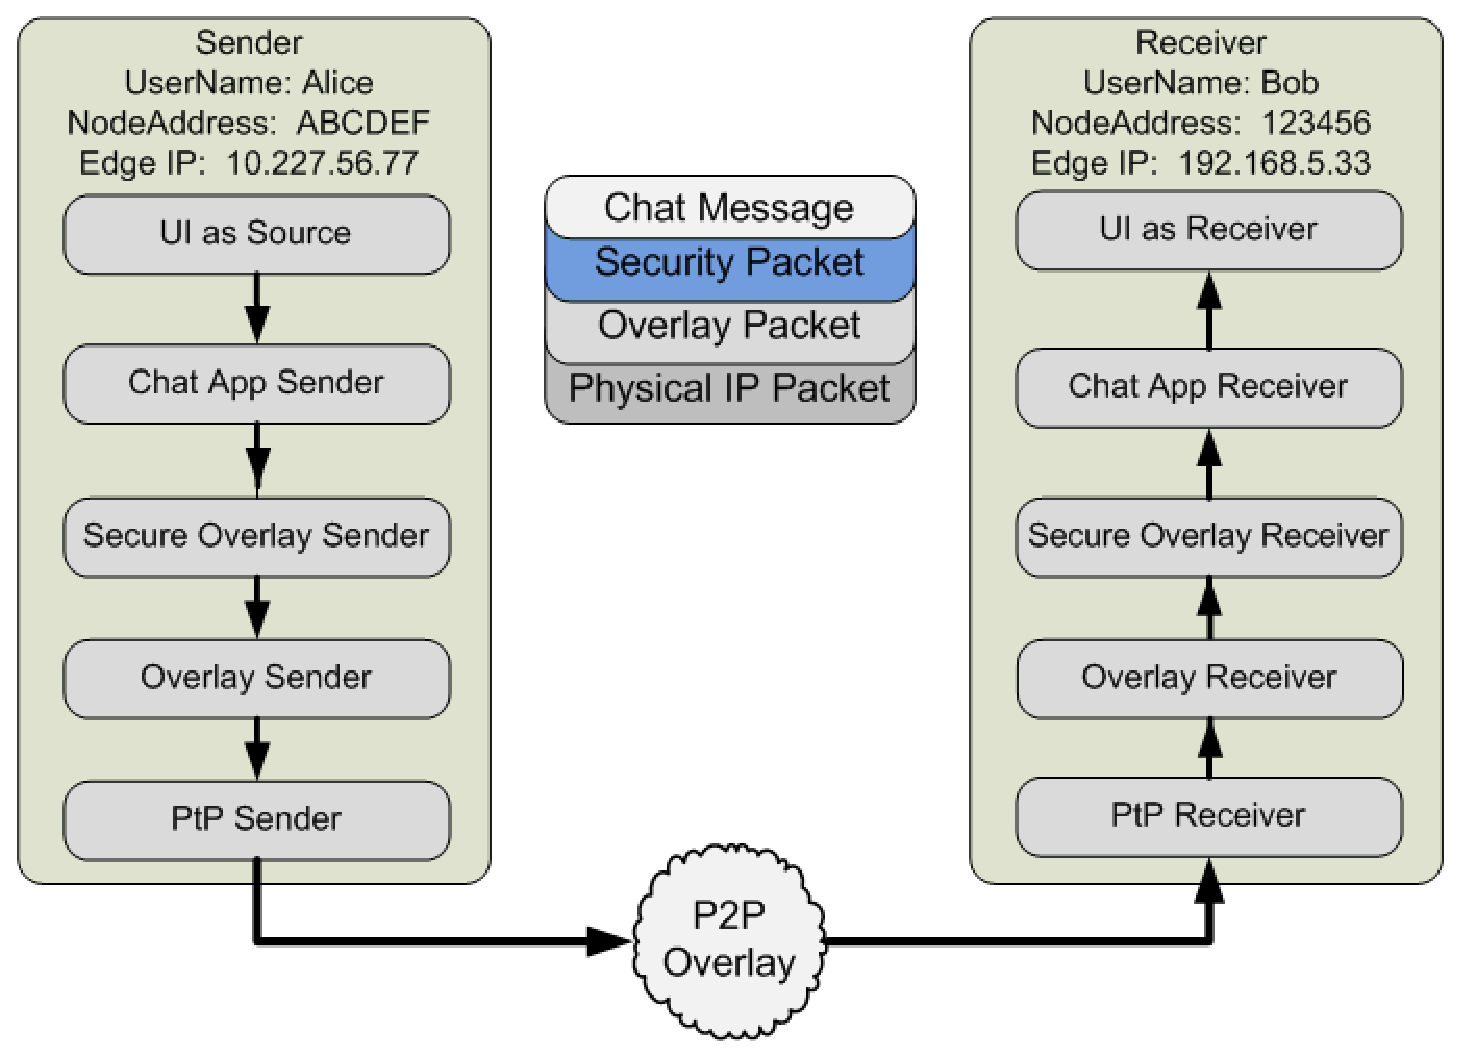
\includegraphics[width=3.25in]{figs/secure_sender_stack_generic.png.eps}
\caption{An example of the abstraction of senders and receivers using a EtE 
secured chat application.  Each receiver and sender use the same abstracted
model and thus the chat application requires only high-level changes, such
as verifying the certificate used is Alice's and Bob's, to support security.}
\label{fig:security_filter}
\end{figure}

In the use of a filter approach, this requires one change to the core software,
such that it verifies the identity of the remote side prior to allowing packets
to traverse the session.  In our system, we did this by means of a callback,
which presents the underlying sending mechanism, EtE or PtP, and the overlay
address stored in the certificate.  The receiver of the callback can attempt to
cast it into known objects, if successul, it will compare the overlay address
with the sender type.  If unsuccessful, it ignores the request.  If any
callbacks return that the sender does not match the identifier, the session is
immediatley closed.

In addition, this requires one change to the core software, such that it
verifies that the sender of the message matches the remote sides certificate or
agreed upon address.  In all cases, this occurs during session establishment.
Though during our implementation of this feature, we realized that our VPN did
not verify that the overlay address of the sender matches its assigned IP
address.  Similarly, if the address is not recorded in a DHT operation, there
will be no way to identify who may have placed a malicious data packet.
Likewise, a PtP link should not be able to affect another PtP link, for
example, by means of a malicious shutdown message.

Finally, there is the issue of identity.  A certificate must uniquely identify
a user and match them to a specific resource.  If a CA were to sign a
certificate without any form of machine identification, a user or system could
easily impersonate others.  This is why all certificates used for web sites
include the web sites domain.  When a user accesses a website, the browser can
verify that the domain name listed in the certificate matches the domain being
accessed by the users, all performed without user interaction.  In environments
with NATs, dynamic IP addresses, or portable devices, assigning a certificate
to a domain name or IP address will be a hassle as it contrains mobility and
the type of users in the system, furthermore, most users are unaware of their
IP address and changes to it.  Instead, a certificate are signed against the
users P2P address.  In doing so, once a PtP or EtE links has been established,
the two nodes must exchange their node addresses and if they do not match the
address on the verified certificate they will be dropped.  This mechanism
allows the same certificate to be used portably.

\subsection{Overheads of Overlay Security}

When applying an additional layer to a P2P system, there will be obvious
overheads in terms of time to become connected to the overlay.  Other less
obvious effects will be throughput, latency, and processing overheads, this is
primarily due to the use of the P2P system over a wide area network, where the
latency and throughput limitations due to the network conditions between two
points will make the overhead of security negligible except in the case of
bootstrapping due to additional round trip messages used for forming a secure
connection.

\begin{figure}[ht]
\centering
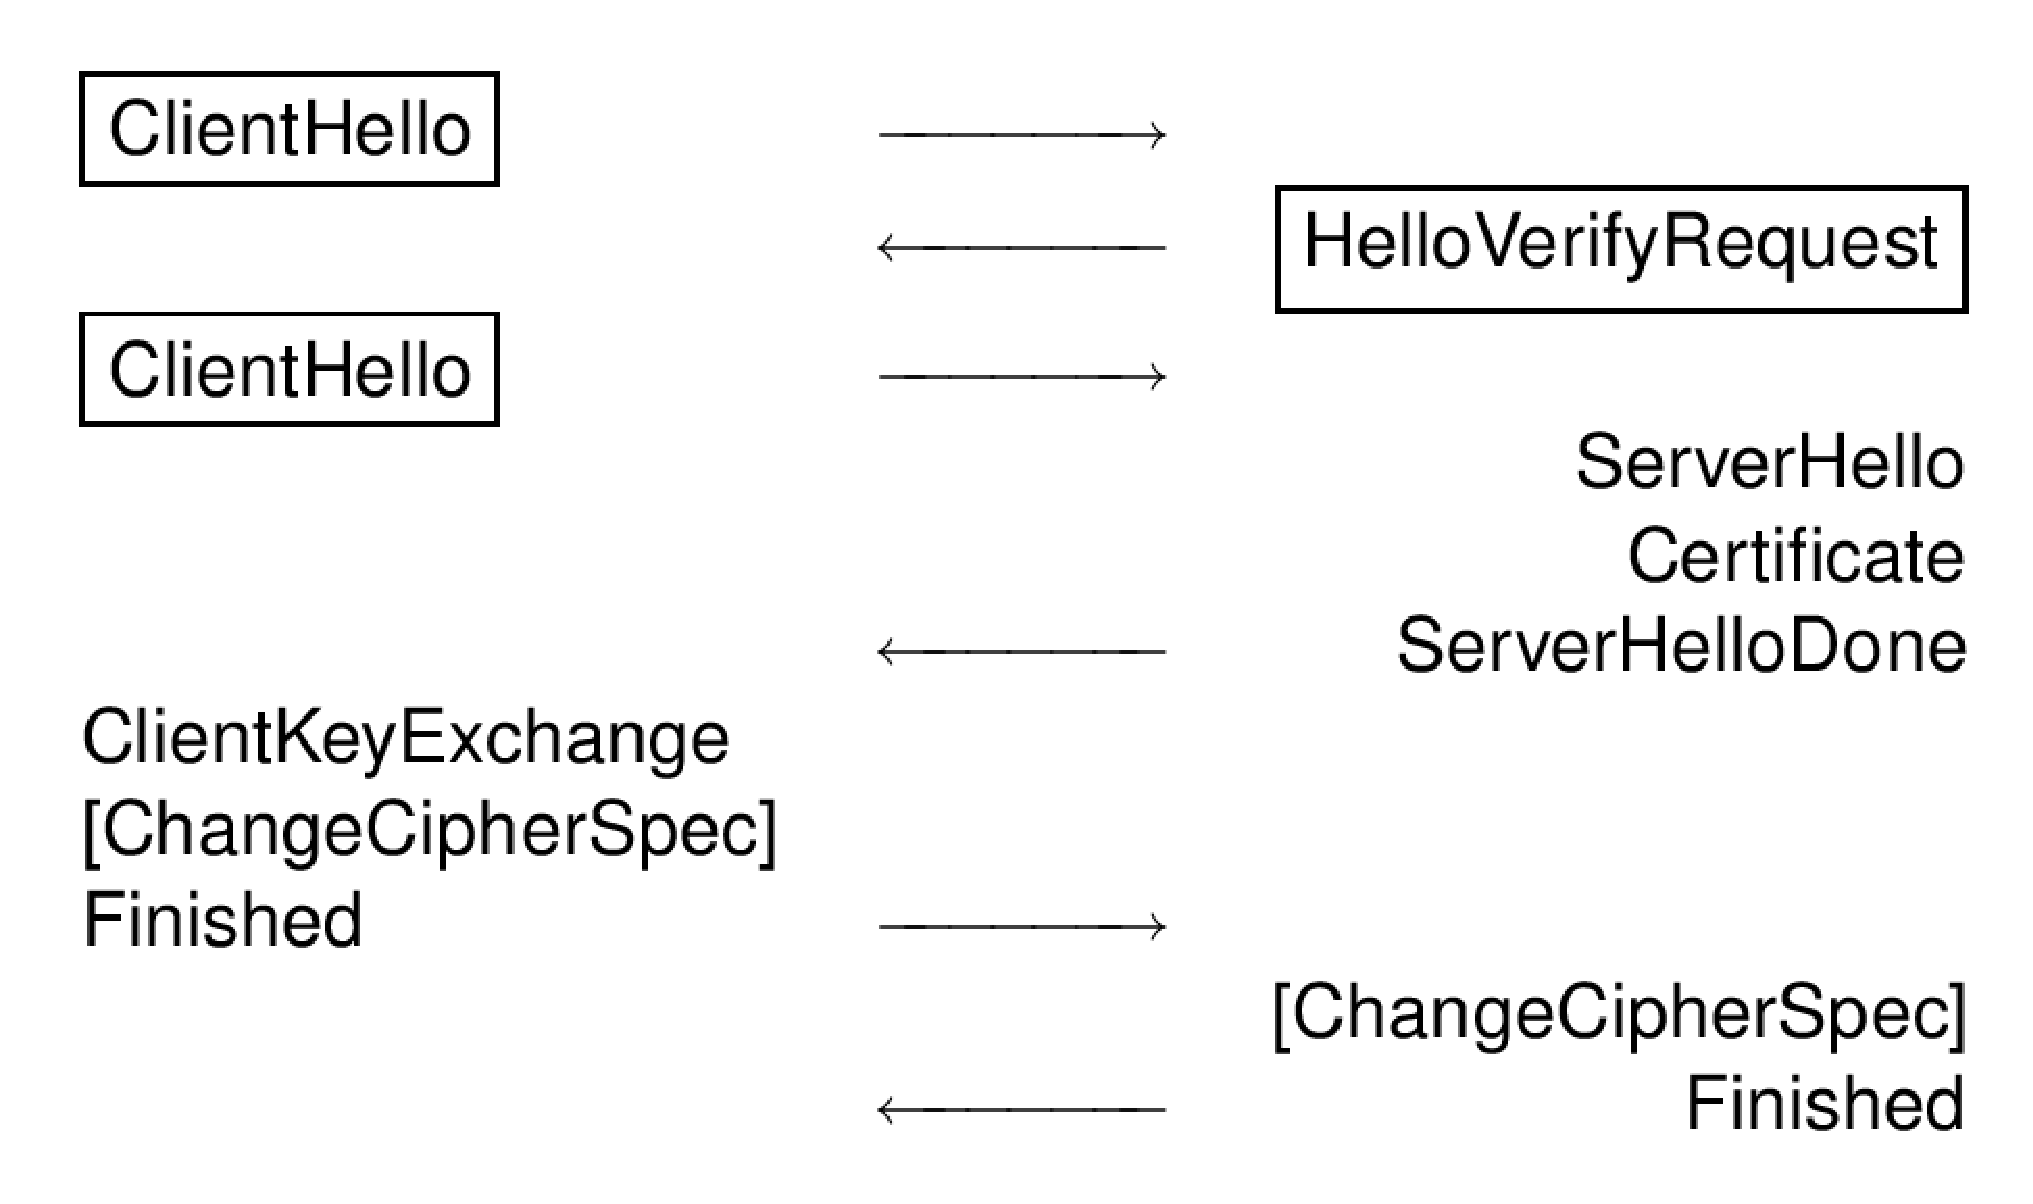
\includegraphics[width=2.5in]{figs/dtls.eps}
\caption{DTLS handshake}
\label{fig:dtls}
\end{figure}

For example, consider the DTLS handshake as presented in Figure~\ref{fig:dtls},
which consists of 6 messages or 3 round trips.  Clearly, this will have an
effect on how quickly an overlay can bootstrap.  To a lesser degree, with more
messages during bootstrap, the probability one drops is higher, which could
have a effect, though possibly negligible, on time to connect.  To evaluate
these concerns, we have employed both simulation and real system experiments.

Both the simulation and real system use the base code of Brunet.  The
simulation code differs from the deployed software in that time is based upon a
virtual timer incremented based upon an event schedule.  In addition, the
simulation environment uses an abstracted transport layer similar to UDP though
all communication is kept within the program and it does not use the underlying
OS' networking stack.  The simulated transport layer supports timing delays and
random packet dropping.  Both have their advantages though, as simulation
allows faster than real time execution of reasonable sized networks (up to a
few thousand) while still enabling easy debugging.  Testing in a deployment
ensures that the software really works in potentially unfavorable conditions,
which are difficult to duplicate in simulation, such as occassional network
glitches, CPU delays on processing, and other random difficult to ascertain
events.

Both the simulation and deployed environment can be used to test the delay
incurred for bootstrapping a single node into an existing, stable network,
while the simulation is the only feasible way to measure how long it takes to
bootstrap a completely new network.  Both simulation evaluation set the delay
between end points to be a common constant and test various network sizes
ranging from 2 to 1,024 in powers of 2.  While the deployment evaluation is
limited in such fine grained testing due to the environment used:
PlanetLab~\cite{planetlab}.  PlanetLab provides nearly 1,000 resources
distributed across Earth.  In practical application, though, roughly 40\% of
the resources are unavailable at any given time and the remaining behave
somewhat unpredictably.  In fact, most of the bugs in our software are detected
early by doing tests on PlanetLab.

\subsection{Discussion}

\section{Handling User Revocation in a Secure Overlay}
\label{revocation}

Unlike decentralized systems that use shared secrets, in which the creator of
the overlay becomes powerless to control malicious users, a PKI enables the
creator to effectively remove malicious users.  Typical PKIs either use a
certificate revocation list (CRL) or online certificate verification protocols
such as Online Certificate Status Protocol (OCSP).  These approaches require a
dedicated service provider in order to verify a certificate, if the service
provider is offline, an application  can only rely on historical information to
make a decision on whether or not to trust a link.  In a decentralized system,
these features can be enhanced so not to rely on a single provider.  In this
section, we present two mechanisms of doing so: storing revocations in the DHT
and performing overlay broadcast based revocations.

\subsection{DHT Revocation}

The DHT provides revocation similarly to the approach of OCSP or CRLs, where
user can either query a service provider to obtain the validity of one or more
certificates.  A revocation is stored in the DHT by signing the hash of a
certificate and the time stamp of revocation and storing all three in the DHT
at the key formed by the hashing of the certificate.  In doing so, revocations
will be uniformly distributed across the overlay, not relying on any single
entity.

The problem with the DHT approach is that it does not provide an event
notification for members currently communicating with the peer.  While peers
could continue to poll the DHT to determine a revocation, doing so is
inefficient.  Furthermore, a malicious peer, who has a valid but revoked
certificate could force every member in the overlay to query the DHT,
negatively affecting the DHT nodes storing the revocation.

\subsection{Broadcast Revocation}

Broadcast revocation can be used to address the deficiencies of DHT revocation.
As a topic of many papers prior~\cite{broadcast, chord_broadcast}, a structured
overlay can be used without additional state to perform efficient broadcasts
from any point in the overlay to the entire overlay.  The form of broadcast can
be used to perform to notify the entire overlay immediately about a new
revocation.  In these papers, analysis and simulations have shown that the
approach can be completed in $O(\log^2 n)$ time.

\begin{figure}[ht]
\centering
\includegraphics[width=2.5in]{figs/tree.eps}
\caption{Broadcast performing a complete overlay broadcast}
\label{fig:tree}
\end{figure}

Our modified algorithm as illustrated in Figure~\ref{fig:tree} utilizes the
organization of a structured system with a circular address space that requires
peers be connected to those whose node addresses are the closest to their own,
features typical of 1-d structured overlays including Chord~\cite{chord},
Pastry~\cite{pastry}, and Symphony.  Using such an organization, it is possible
to do perform a broadcast with no additional state.  To perform a broadcast,
each node performs the following recursive algorithm:
\begin{algorithmic}
\STATE {\bf BROADCAST(start, end, message)}:
  \STATE RECEIVE(message)
  \FOR{$i$ in length(connections)}
    \STATE n\_start $\gets$ ADDRESS(connections$[i]$)
    \IF {n\_start $\not\in$ $[$start, end$)$}
      \STATE continue
    \ENDIF
    \STATE n\_end $\gets$ ADDRESS(connections$[i+1]$)
    \IF {n\_end $\not\in$ $[$start, end$)$}
      \STATE n\_end $\gets$ end
    \ENDIF
    \STATE msg $\gets$ (BROADCAST, n\_start, n\_end, message)
    \STATE SEND(connections$[i]$, msg)
  \ENDFOR
\end{algorithmic}
with ``connections'' as a circular list of connections in non-decreasing order
from the perspective of the node performing the current recursive, broadcast
step.

In this algorithm, broadcast initiator uses its own address as the start and
end, thus the broadcast will span the entire overlay after completing recursive
calls at each connected node.  A recursive end, ``n\_end'', must be inside the
region between ``start'' and ``end'', thus if the connection following the
current sending connection, ``connections$[i+1]$'', is not in that region, it
will only broadcast up to ``end'' and not the address specified by that
connection.  Finally, nodes, who have a connection to the malicious peer, will
end the connection prior to accidentally forwarding the message to the peer by
receiving and acting upon the revocation prior to forwarding the message.  To
summarize, the overlay is recursively partitioned amongst the nodes at each hop
in the broadcast.  By doing so, all nodes receive the broadcast without
receiving duplicate broadcast messages.

\subsection{Evaluation of Revocation Models}

%Figure~\ref{fig:revocation} presents the time required to perform a revocation
%using the simulator described in Section~\ref{security.evaluation}.  After the
%system establishes steady state, a random node is selected to be revoked.  This
%evaluation measures the time to perform such a revocation.  In the case of a
%broadcast a broadcast revocation, this is the time for a message to be
%distributed to the entire overlay, whereas in the case of DHT, it is the time
%to perform the DHT insertion.

%The results seem to indicate that in terms of time, network size and bandwidth
%scale well together.  In contrast, the network traffic scales significantly
%better in DHT experiments, though the approach can be inefficient for
%environments consisting of malicious and colluding peers.  In a DHT revocation,
%revoked peers can attempt to connect with new peers who do not know about the
%revocation, causing each of them to query the DHT to discover the revocation.
%If this becomes the case, the DHT method will quickly become inefficient.  On
%the other hand, the broadcast cannot ensure that all nodes receive the message,
%due to overlay network stability issues, peers may not be included in the
%broadcast.  As such the best approach may be to store a revocation in the DHT
%but notify all peers of a revocation via a broadcast.  Broadcast is efficient
%with bandwidth both for the broadcasting peer and the overlay.  The
%broadcasting peer only sends out as many packets as connections it has, while
%the tree formed by broadcast spans exactly N-1 connections.  In other words,
%the network traffic required to do a broadcast on this tree is the minimum
%amount of communication necessary to reach all nodes in the broadcast range.

\begin{figure*}[ht]
\centering
\includegraphics[width=3in,angle=-90]{figs/groupvpn.ps}
\caption{Process in bootstrapping a new GroupVPN instance.}
\label{fig:groupvpn}
\end{figure*}

\subsection{Discussion}

In contrast to the DHT solution, broadcast revocation occurs only once and does
not leave state behind.  Thus the broadcast is not a complete solution, new
peers to the overlay or those who missed the broadcast message will be unaware
of a revocation.  Furthermore, if an overlay is shared by many VPNs, it may
prevent overlay broadcasting or itself may be inefficient.  

The DHT solution by itself may also not sufficient as revocations may be lost
over time as the entries must have their leases renewed in the DHT.  To address
this condition, each peer maintains a local CRL and the owner of the overlay
can occasionally send updates to the CRL through an out of band medium, such as
e-mail.  A better long term solution may be the use of a gossip protocol so
that peers can share their lists with each other during bootstrapping phases.

A key assumption in using these is that a Sybil~\cite{sybil}, or collusion
attack, is difficult in the secured overlay.	 If a Sybil attack is successful,
both a DHT and broadcast revocation may be unsuccessful, though peers could fix
this problem by obtaining the CRL out of band.  In addition, previous
work~\cite{secure_routing} has described decentralized techniques to limit the
probability of such attacks from occurring.  In our approach, the use of
central authority to review certificate requests can be used to limit a single
user from obtaining too many certificates as well as ensuring uniform
distribution of that user's P2P addresses, further hampering the likelihood of
a Sybil attack.  The ability to automate this is left as future work.

\section{Managing and Configuring the VPN}
\label{groupvpn}

While the PKI model applies cleanly to P2P models, setting up, deploying, and
then maintaining security credentials can easily become a non-negligible task,
especially for non-experts.  Most PKI-enabled systems require the use of
command-line utilities and lack methods for assisting in the deployment of
certificates and policing users.  In order to facilitate use in real systems
with non-experts, it is important to have an easy to use framework.  Our focal
solution to this issue is a partially automated PKI reliant on a group based
web interface distributable in forms of Joomla add-ons as well as a virtual
machine appliance.  In this environment, groups can share a common site with
each group having their own unique CA.  Although this does not preclude other
methods of CA interaction, experience has shown that it provides a model that
is satisfactory for many use cases.

A group based Web 2.0 environment enables low overhead configuration of
collaborative environments.  The roles in a group environment can be divided
into administrators and users.  Users have the ability to join and create
groups; whereas administrators define network parameters, accept or deny join
requests, remove users, and promote other users to administrators.  By applying
this to a VPN, the group environment provides a wrapper around a public key
infrastructure (PKI), where the administrators of the group act as the
certificate authority (CA) and the members have the ability to obtain signed
certificates.  Elaborating further, when a user joins a group, the
administrator can enable automatic signing of certificates or require prior
review; and when peers have overstayed their welcome, an administrator can
revoke their certificate by removing them from the group.  Revocations are
stored on the site as a CRL (certificate revocation list) and when they occur
are broadcast onto the overlay and inserted into the DHT of the respective
overlay.  Though for these forms of systems a user revocation list as opposed
to a CRL simplifies revocation, since users and not individual certificates
will be revoked.

Administrators of a group configure the VPN address range, namespace, security,
and the ability to specify reuse of an existing overlay or a list of user
managed nodes.  When a user has been accepted into the group, they are able to
download VPN configuration data, which can be seamlessly added to the VPN by
running the VPN configuration process.  In addition to IP address range,
namespace, and security options, the configuration data also contains the group
website's address and a shared secret.  The shared secret uniquely identifies
the user, so that the website can automatically sign the certificate or enqueue
it so the administrator can manually sign it.  Certificate requests consist of
a public key and the user's shared secret and are sent over HTTPS to the web
server.  The website creates and signs a certificate request based upon the
public key and the user's relevant information ensuring that users cannot trick
the website into signing malicious data.  Upon receiving the signed
certificate, peers are able to join the private overlay and VPN enabling secure
communication amongst the VPN peers.  The entire bootstrapping process
including address resolution and communication with a peer is illustrated in
Figure~\ref{fig:groupvpn}.

There are many ways of implementing and hosting the web site.  For example,
Google offers free hosting of Python web applications through Google Apps, but
this requires that the user owns a domain.  Alternatively, the user could host
the group site on a public VN, peers interacting with the GroupVPN would need
to connect with the public VN in order to create an account, get the
configuration data, and to sign their certificate at which point they could
disconnect from it.  This does not preclude the use of other social mediums nor
a central site dedicated to the formation of many GroupVPNs.  Many GroupVPNs
can share a single site, so long as the group members trust the site to host
the CA private key.

\section{Evaluation of VPN Models}
\label{evaluation}

This experiment explores bandwidth and latency in a distributed VPN system to
motivate the usage of P2P links in a VPN.  The VPNs used include our GroupVPN,
OpenVPN, and Hamachi.  OpenVPN represents a typical centralized VPN, while
Hamachi represents a well-tuned P2P-link VPN.  The evaluation was performed on
Amazon EC2 using small instance sized Ubuntu i386 instances to create various
sized networks ranging from 1 to 32.  OpenVPN uses an additional node as the
central server and Hamachi has an upper bound of 16 due to limitations in the
Linux version at the time of this evaluation.  To perform bandwidth tests, the
instances are booted and query an NFS for the list virtual IP addresses, peers
are ordered such that half the peers are act as clients and the other half the
peers creating a 1 to 1 mapping between all sets.  Latency and bandwidth tests
are performed using netperf's request-reply and streaming tests respectively.
Prior to the start of the tests, peers have no knowledge of each other, except
the virtual IP addresses, thus connection startup costs are included in the
test.  Tests are run for 10 minutes diluting the connection initiation overhead
but represent an example of real usage.  Results from the clients are polled at
all locations and averaged together, though the OpenVPN server is measured
separately.  GroupVPN and OpenVPN use authenticated 128-bit AES, while Hamachi
does not allow configuration of the security parameters and uses the default
Hamachi settings, 256-bit AES.

\begin{figure}[ht]
\centering
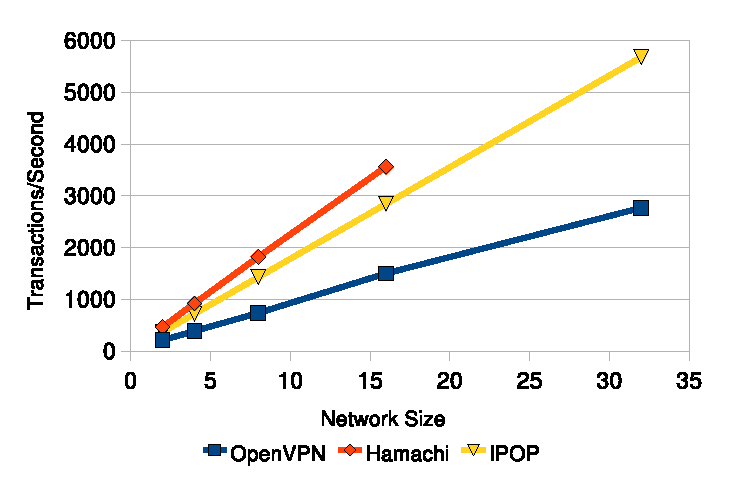
\epsfig{file=figs/latency.eps, width=2.25in}
\caption{System transaction rate for various VPN approaches.}
\label{fig:latency}
\end{figure}

\begin{figure}[ht]
\centering
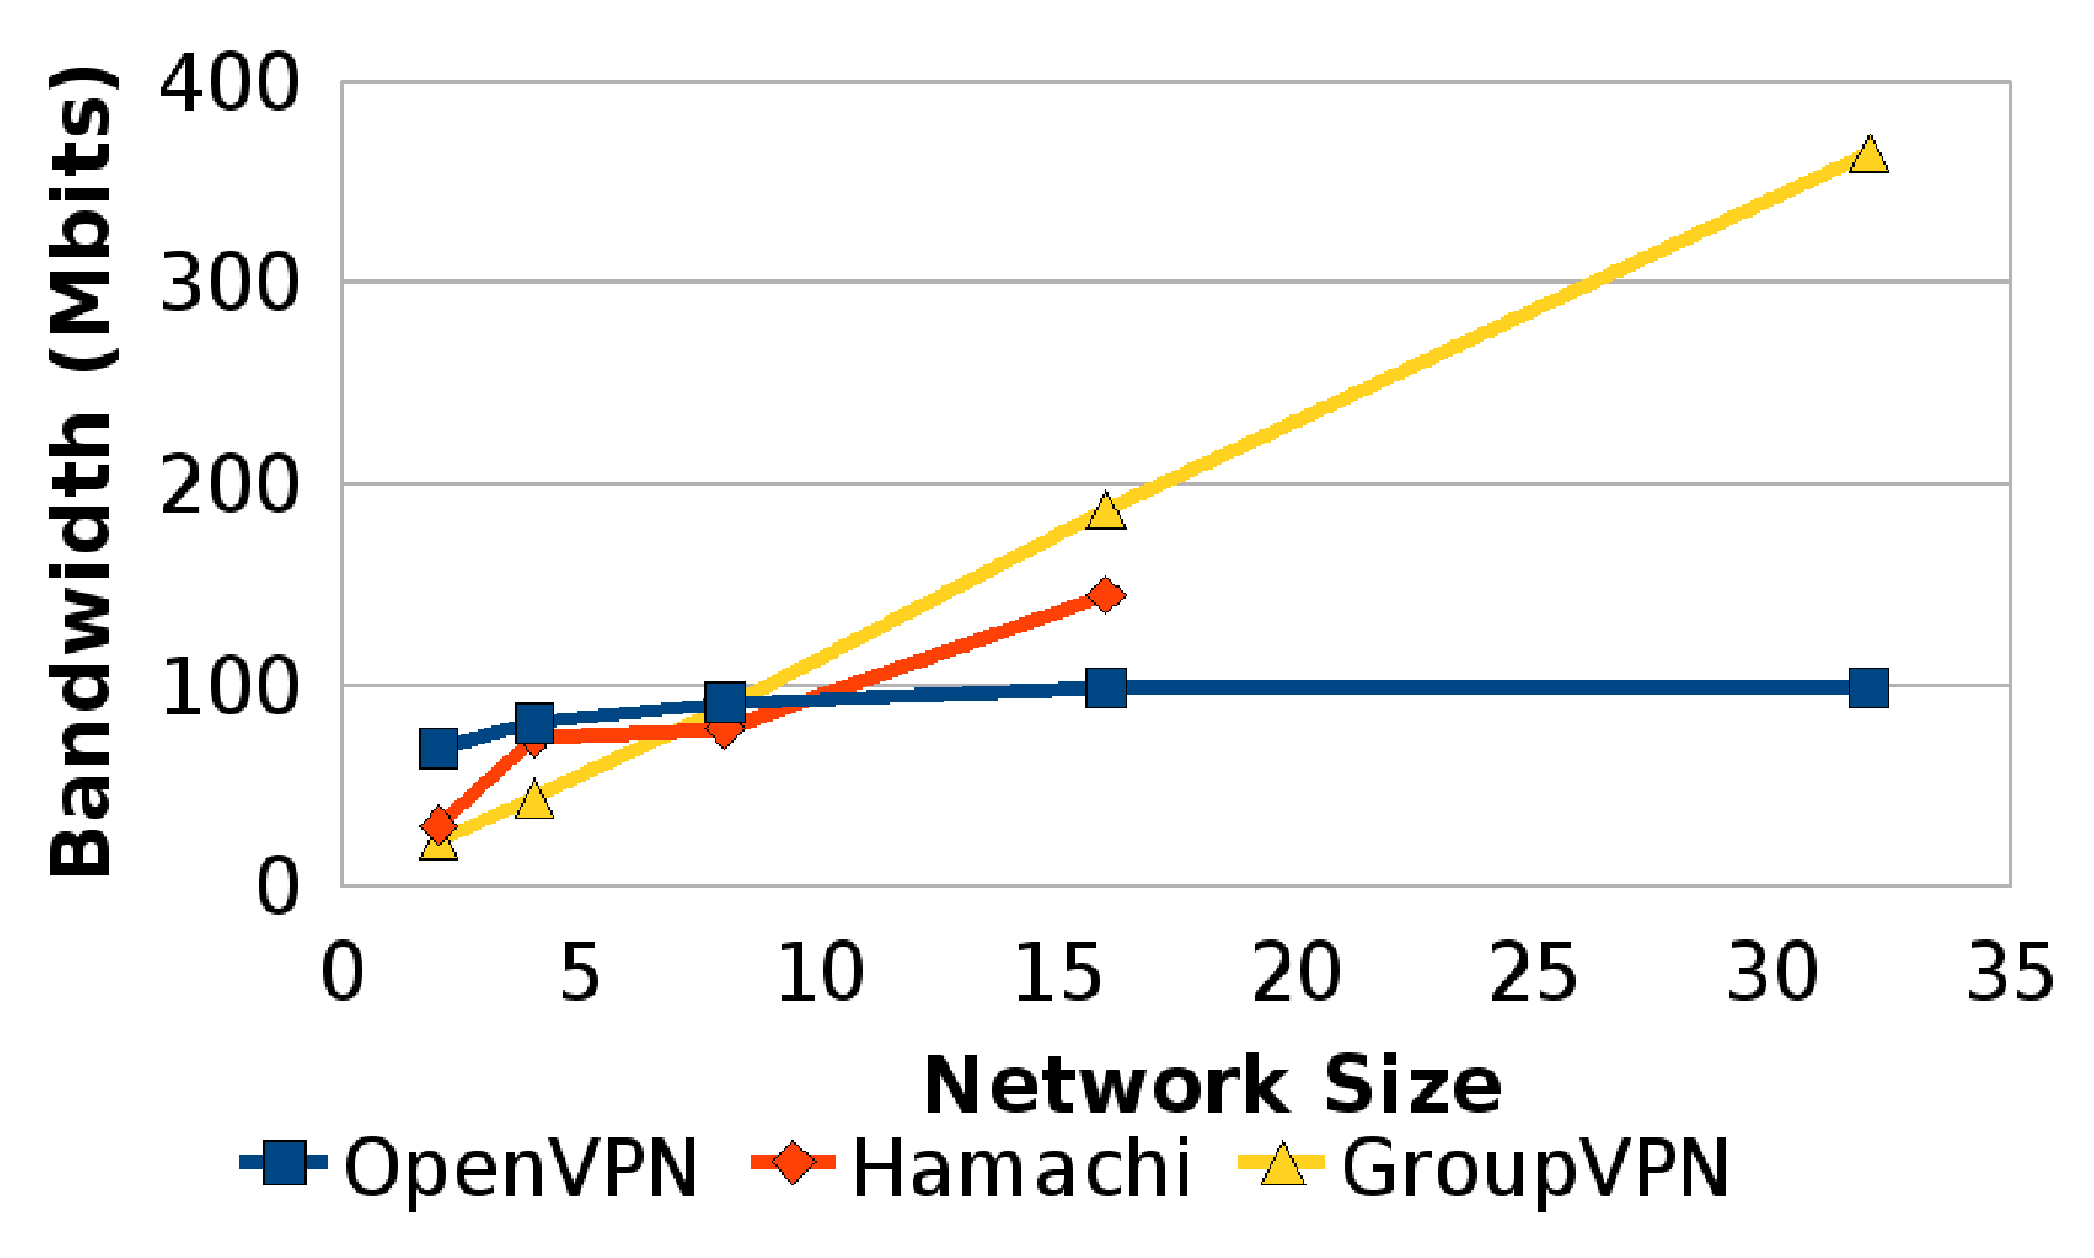
\epsfig{file=figs/bandwidth.eps, width=2.25in}
\caption{System bandwidth for various VPN approaches.}
\label{fig:bandwidth}
\end{figure}

Figures \ref{fig:latency} and \ref{fig:bandwidth} present the results for
latency and bandwidth respectively.  Latency is measured in transactions of
successful request/reply messages.  In the latency test, it is obvious that
having the central server increases the delay between the client and server and
the results degrade more quickly as additional peers are added to the system.
In small systems, OpenVPN shines probably due to optimized software, though as
the system grows, the system bandwidth does not.  By the time 8 peers have
entered into the system, both decentralized approaches perform better than the
OpenVPN solution.  To summarize, decentralized VPN approaches provide better
scalability, which can be immediately noticed by low latency times and, as the
system grows, available bandwidth.

\section{Related Work}
\label{related_work}

\subsection{VPNs}

Hamachi~\cite{hamachi} provides central group management and a security
infrastructure through a Web interface.  Their security system has gone through
two revisions as documented in~\cite{hamachi_security}.  Initially peers learn
of each other through Hamachi's central system, which leads to the creation of
secure links.  In their original approach, they use a system similar to a Key
Distribution Center (KDC), which requires that all security sessions initiate
through Hamachi's central servers.  In the latest version, this model has been
retained but with the addition of an external PKI, which avoids the
man-in-the-middle attack but with has the additional cost of maintaining both
an external CA and certificate revocation list (CRL).  Hamachi also supports
STUN, or NAT hole punching, and TURN style NAT traversal, though TURN requires
the use of Hamachi's own relay servers.  Because Hamachi is closed, it disables
users from hosting their own infrastructures including session management and
relay servers.

\subsection{P2P Systems}

BitTorrent~\cite{bittorrent_security}, a P2P data sharing service,  supports
stream encryption between peers sharing files.  The purpose of BitTorrent
security is to obfuscate packets to prevent traffic shaping due packet
sniffing. Thus BitTorrent security uses a weak stream cipher, RC4, and lacks
peer authentication as symmetric keys are exchanged through an unauthenticated
Diffie-Hellman process.

Skype~\cite{skype} provides decentralized audio and video communication to over
a million concurrent users.  While Skype does not provide documentation
detailing the security of its system, researchers~\cite{skype_auth,
skype_overview} have discovered that Skype supports both EtE and PtP security.
Though similar to Hamachi, Skype uses a KDC and does not let users setup their
own systems.

As of December 2009, the FreePastry group released an SSL enabled
FreePastry~\cite{pastry}.  Though relatively little is published regarding
their security implementation, the use of SSL prevents its application for use
in the overlay and for overlay links that do not use TCP, such as relays and
UDP.  Thus their approach is limited to securing environments that are not
behind NATs and firewalls that would prevent direct TCP links from forming
between peers.

\subsection{Certificate Authorities}

The RobotCA~\cite{robotca} provides an automated approach for decentralized
PKI.  A RobotCAs receives request via e-mail, verifies that the sender's e-mail
address and embedded PGP key match, signs the request, and mails it back to the
sender.  RobotCAs are only as secure as the underlying e-mail infrastructure
and provide no guarantees about the person beyond their ownership of an e-mail
address.  A RobotCA does not provide features to limit the signing of
certificates nor does it provide user-friendly or intuitive mechanisms for
certificate revocation.

\section{Conclusions}
\label{conclusions}

This paper describes a novel approach to VPNs utilizing structured overlays to
deal with organization, public overlays for connectivity, private overlays for
security, and collaborative environments for configuration and management.
This paper extends our previous work, IPOP, a P2P virtual network system, to
support user-friendly approaches for users to create and manage their own IPOP
systems with security.  To do this, each IPOP system bootstraps into its own
unique P2P overlay.  This approach not only enables significantly more secure
IPOP deployments but also enables for more efficient overlay multicast and
broadcast and the cost of doing so amounted to only a few hundred lines of
code.

The use of service overlays significantly improves performance and maintenance
from other structured overlay broadcasting techniques that require specialized
organization and in addition, only those involved in the communication are
involved, thus no bandwidth is wasted.  We also presented two models, which can
be used to optimize the use of overlay based broadcast solutions, one
emphasizing balanced bandwidth while the other latency.  As the results
suggest, bandwidth heavy applications such as streaming audio and video will
scale better and benefit more from a balanced bandwidth approach, whereas
discovery systems benefit from the lower latency approach.

Without the functionality of GroupVPN projects like Archer~\cite{archer}, would
be impractical.  Archer consists of over 500 resources from 5 different
universities, including University of Florida, Florida State University,
Northeastern University, University of Minnesota, and University of Texas.  In
the past year, since Archer came online, over 100 unique users have contributed
and taken advantage of the voluntary computing cycles.  A new user to the
system begins by creating an account at \url{Grid-Appliance.org} and requesting
membership in the Archer GroupVPN group.  Once access has been granted, users
can obtain configuration data used by the Grid Appliance initialization scripts
to seamlessly add resources to the grid.  This method allows independent
submission sites, unlike most grid systems that have a shared submission site,
which require dedicated administrators.  Most users connect to the system using
a pre-configured virtual machine appliance, so that they do not need to be
experts in grid systems to take advantage of Archer.  Enabling this using
decentralized VPNs would be difficult as the user would need to create manual
links to the rest of the system for each new resource.  N2N may work, but the
network size of Archer is larger than the recommendations made by N2N and would
still require the setup of address allocation facilities.  In general, all
existing approaches would fail besides those with centralized components,
because, at the time of this writing, all of Archer's resources are behind
NATs.  Even though centralized could be used, it would require additional
dedicated resources and management, limiting access if the central component
went offline.  

The GroupVPN has been used as the virtual network for the Grid Appliance, which
is the basis of Archer and, in general, enables the enables the creation of
distributed, decentralized, collaborative environments for computing grids.
Recently, a grid at La Jolla Institute for Allergy and Immunology went live
using GroupVPN and Grid Appliance without receiving any technical support from
us.  Researchers at Clemson University and Purdue have opted for this approach
over centralized VPNs as the basis of their future distributed compute clusters
and have actively tested networks of over 700 nodes.

%\small{
\bibliographystyle{IEEEtran}
\bibliography{GroupVPN}
%}

\end{document}
